%!TEX root = ./main.tex
\chapter{Artigos JOSS e BrJG}
\label{artigos}

\section{Artigo JOSS}

O \textit{Mandyoc} é um código em elementos finitos 2-D escrito em C com o objetivo de simular convecção termoquímica de planetas rochosos. Em colaboração com Victor Sacek, Agustina Pesce e Rafael Monteiro da Silva, o \textit{Mandyoc} foi publicado na JOSS (\textit{Journal of Open Source Software}) e pode ser acessado usando o \textit{link} \url{https://joss.theoj.org/papers/10.21105/joss.04070} e o repositório do código está inteiro no \textit{GitHub} no \textit{link} \url{https://github.com/ggciag/mandyoc}. Adicionalmente, a documentação do código está disponível no \textit{link} \url{http://ggciag.github.io/mandyoc/}.

\section{Artigo BrJG}

Em comemoração aos 50 anos do departamento de Geofísica do IAG, o grupo de Tectonofísica produziu um artigo relativo ao desenvolvimento da geodinâmica computacional. O artigo é uma colaboração com Victor Sacek, Naomi Ussami, Agustina Pesce, Claudio Alejandro Salazar-Mora, Edgar Bueno dos Santos, Felipe Baiadori, João Pedro Macedo Silva, Rafael Monteiro da Silva e Tacio Cordeiro Bicudo.

As próximas páginas deste relatório contêm o artigo para revisão (\textit{For Review Only}) submetido à \textit{Brazilian Journal of Geophysics} (BrJG, \url{https://sbgf.org.br/revista/index.php/rbgf}) com o título \textit{Computational geodynamics of South American plate: review and perspectives}.

\includepdf[pages={2-17}, scale=0.8, pagecommand={}, frame]{files/article-proof.pdf}

% Ainda trabalhando na documentação formal do código \textit{Mandyoc} para a publicação do artigo, o manual em inglês vem sendo aprimorado e desenvolvido em torno das necessidades do usuário. Uma versão atualizada desse manual pode ser acessada \textit{online} pelo \textit{link} \url{https://ggciag.github.io/mandyoc/}. A documentação também foi adicionada ao repositório oficial do \textit{Mandyoc} (\url{https://github.com/ggciag/mandyoc}), escrita com a ferramenta \textit{Sphinx} (\url{https://www.sphinx-doc.org/}) e hospedada com o \textit{GitHub Pages}.

% Com a mudança do \textit{Read the Docs} (\url{https://readthedocs.org}) para o \textit{GitHub Pages}, a documentação foi unificada ao código e está mais acessível aos usuários do \textit{Mandyoc}.

% As páginas a seguir mostram a documentação da versão mais recente do código. As mudanças em relação à última versão concentram-se na instalação do \textit{Mandyoc} (\url{https://ggciag.github.io/mandyoc/files/installation.html}) e na inclusão e descrição de \textit{benchmarks} (\url{https://ggciag.github.io/mandyoc/files/benchmarks.html}), que estão disponíveis para execução no repositório do código (\url{https://github.com/ggciag/mandyoc/tree/main/examples}). Ainda, o manual contém pequenas correções gramaticais, em fórmulas e em figuras. A documentação agora só contém informações para simulações em 2D, já que o código para resolver problemas em 3D está sendo aprimorado.

% Os trabalhos de \citet{van1997comparison} e \citet{crameri2012comparison} compõem os dois \textit{benchmarks} que foram adicionados ao capítulo 6 da documentação. O trabalho de \citet{van1997comparison} compara vários métodos de estudo de convecção termo-química 2D que consideram a aproximação de Boussinesq e o número de Prandtl infinito. A \textit{url} direta para os resultados dentro da documentação é \url{https://ggciag.github.io/mandyoc/files/benchmarks.html}. O \textit{benchmark} de \citet{crameri2012comparison} compara resultados que utilizam o método \textit{sticky air} para calcular numericamente a topografia de modelos geodinâmicos e seus resultados também estão disponíveis no \textit{link} \url{https://ggciag.github.io/mandyoc/files/benchmarks.html}.

% 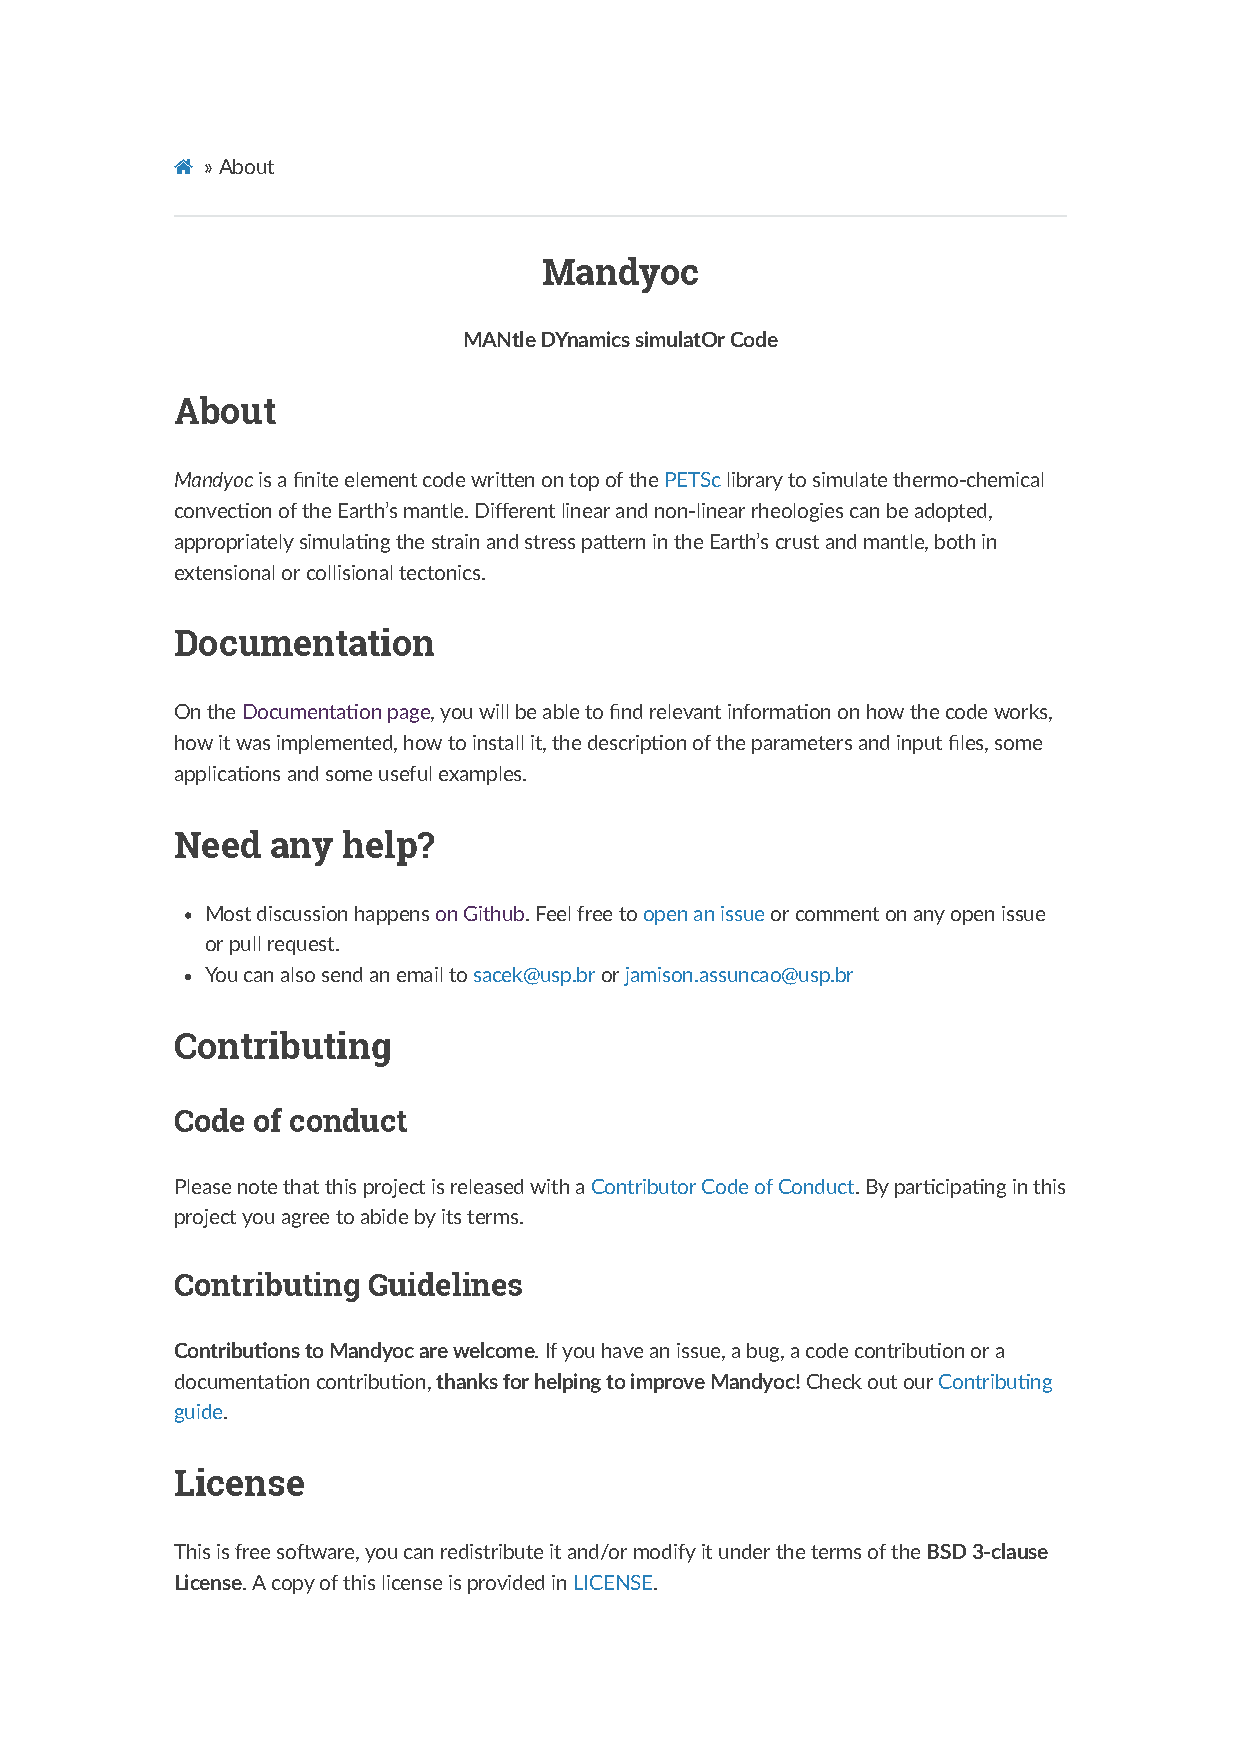
\includepdf[pages=-, scale=0.8, pagecommand={}, frame]{files/0.pdf}
% 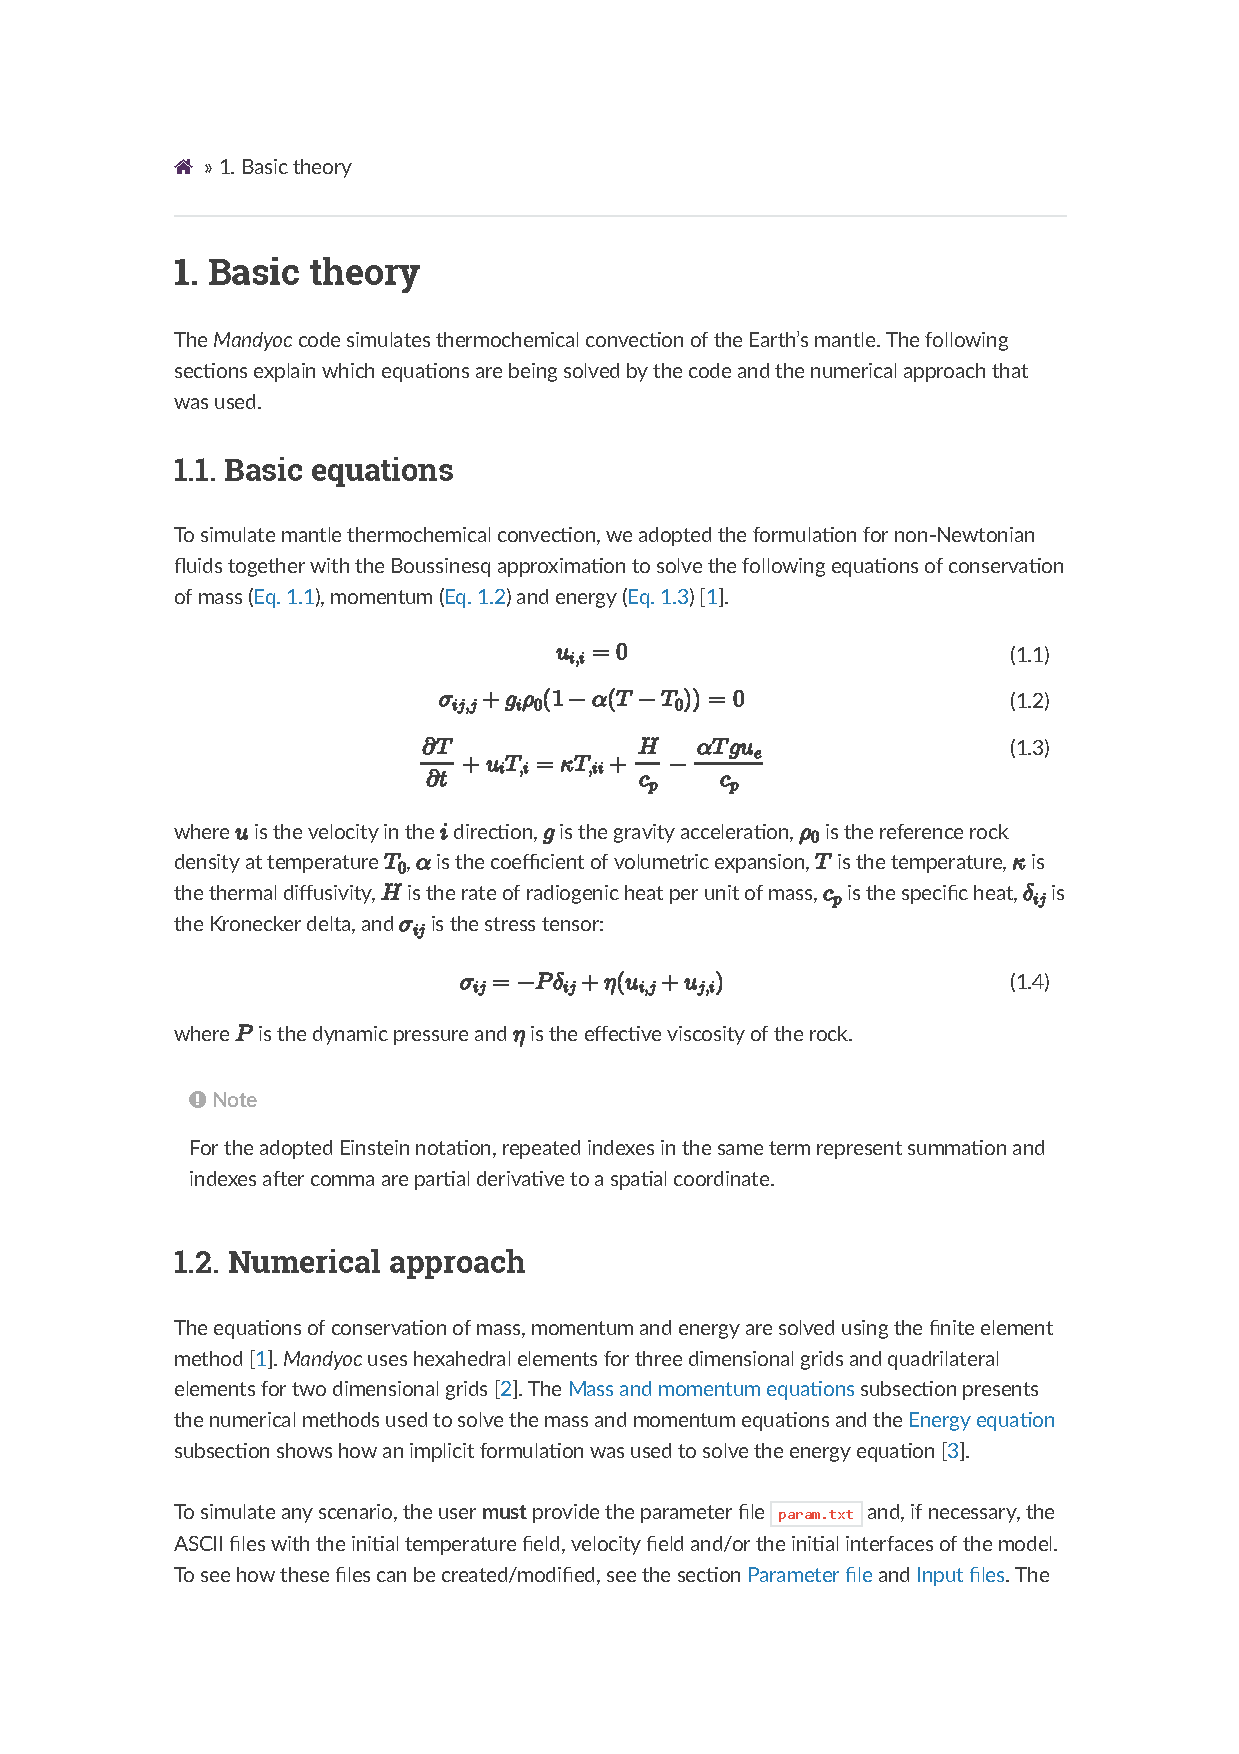
\includepdf[pages=-, scale=0.8, pagecommand={}, frame]{files/1.pdf}
% 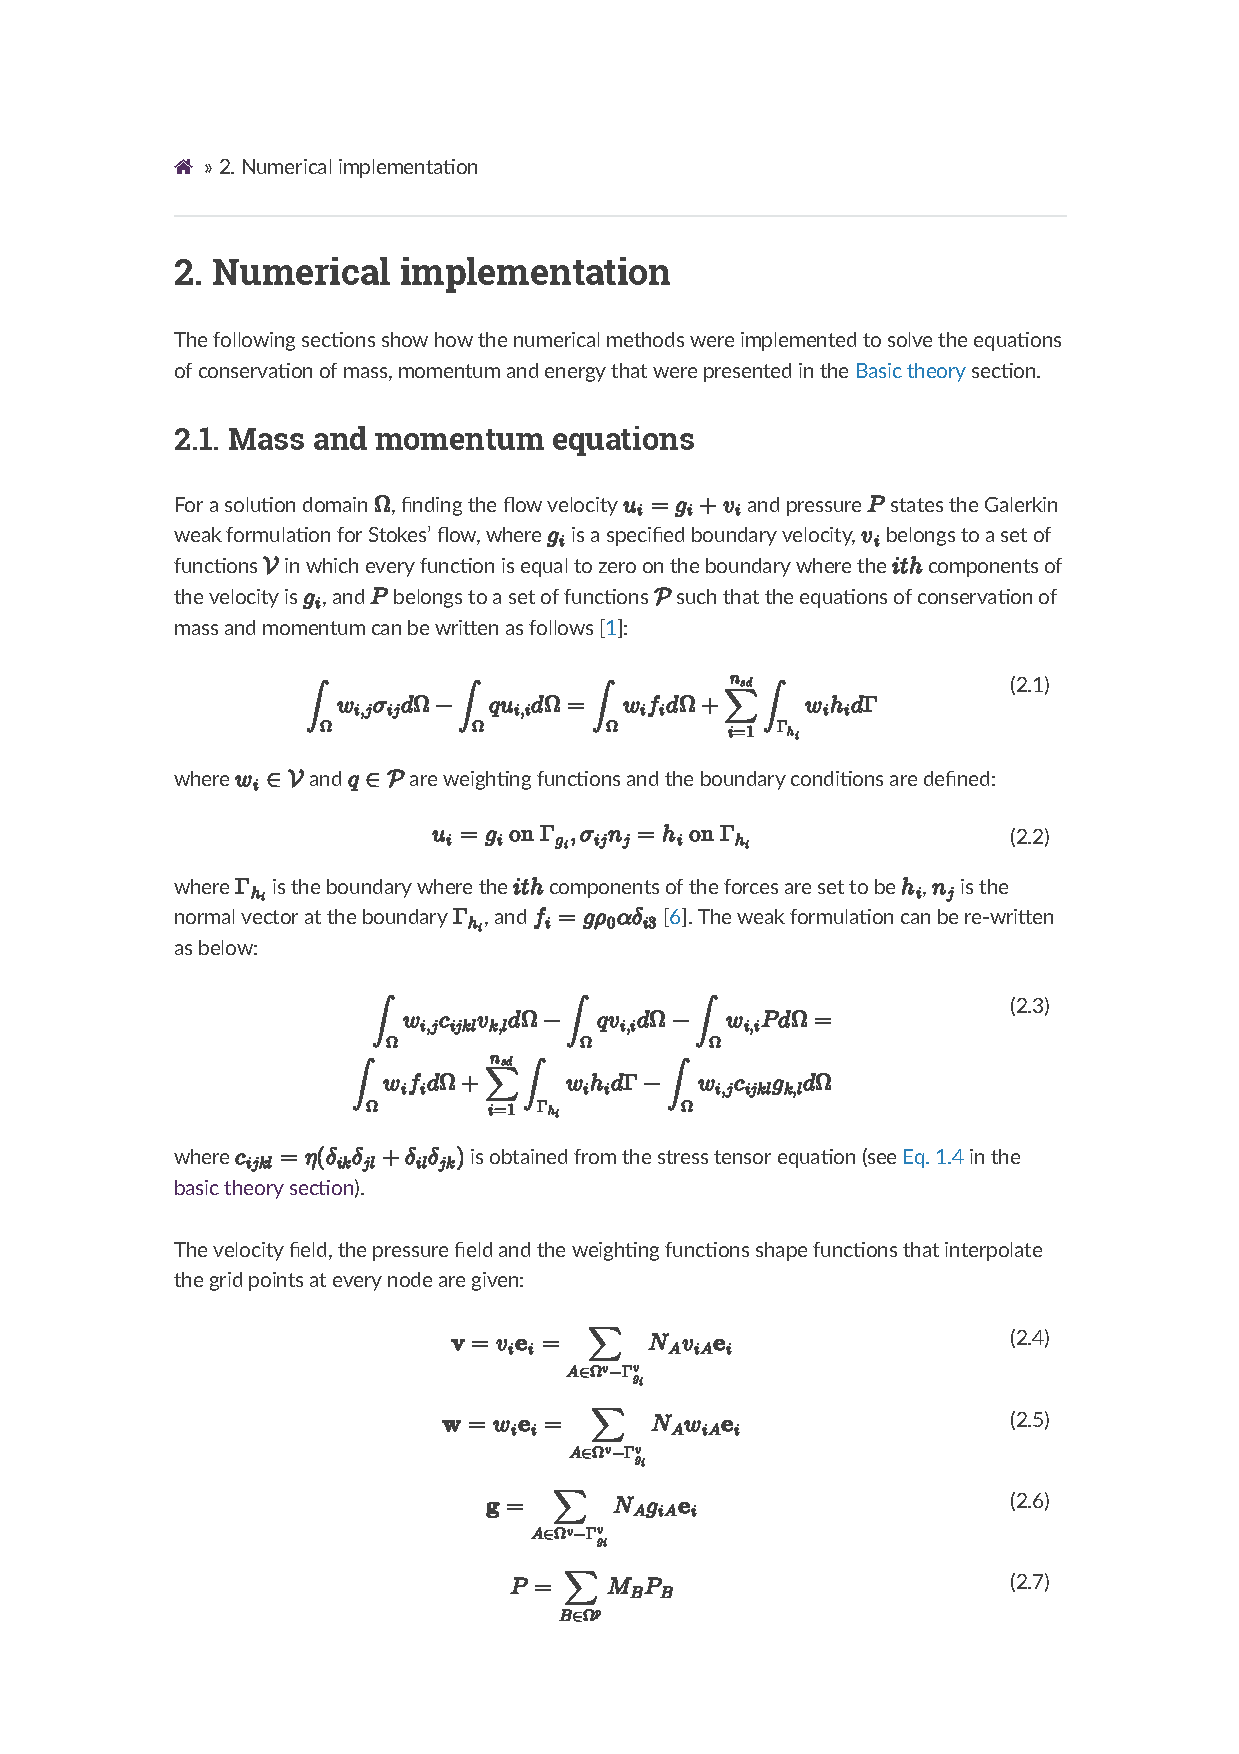
\includepdf[pages=-, scale=0.8, pagecommand={}, frame]{files/2.pdf}
% 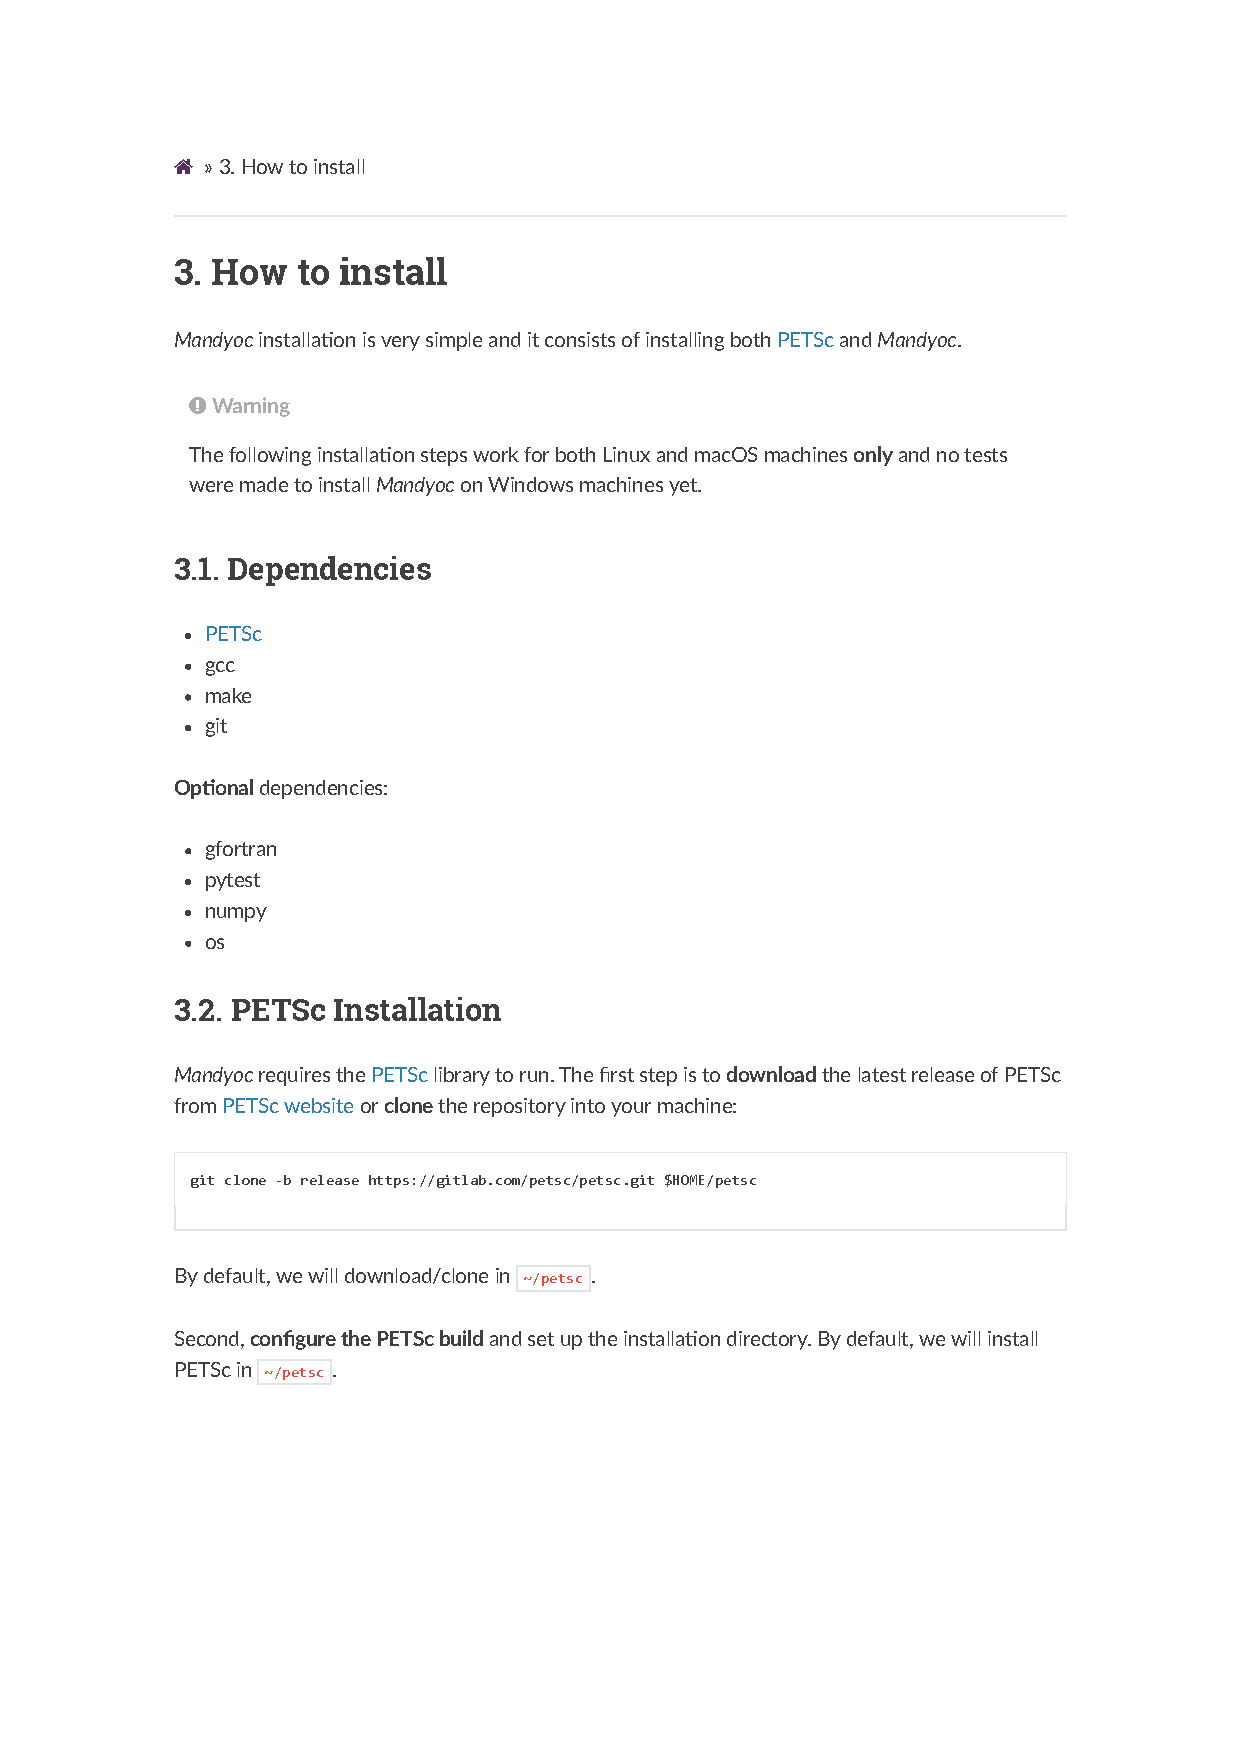
\includepdf[pages=-, scale=0.8, pagecommand={}, frame]{files/3.pdf}
% 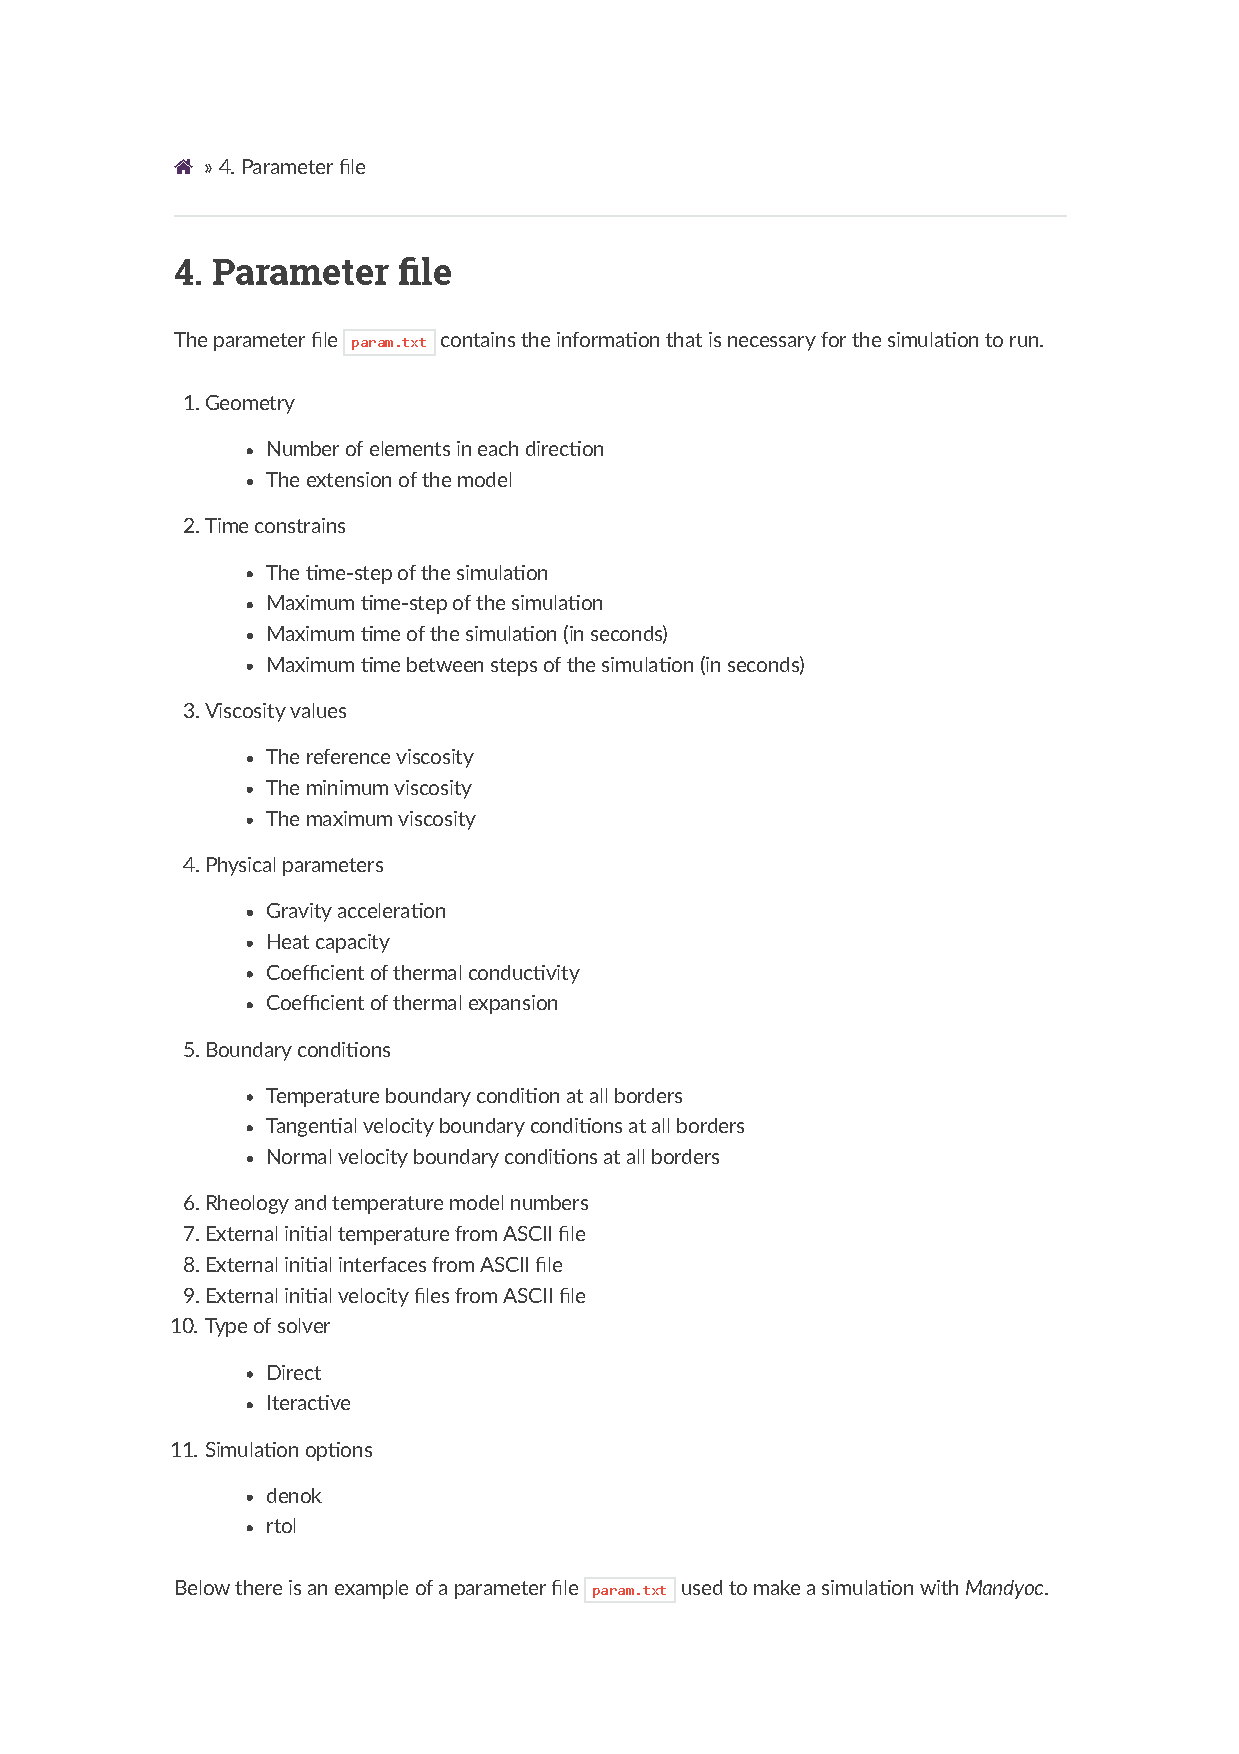
\includepdf[pages=-, scale=0.8, pagecommand={}, frame]{files/4.pdf}
% 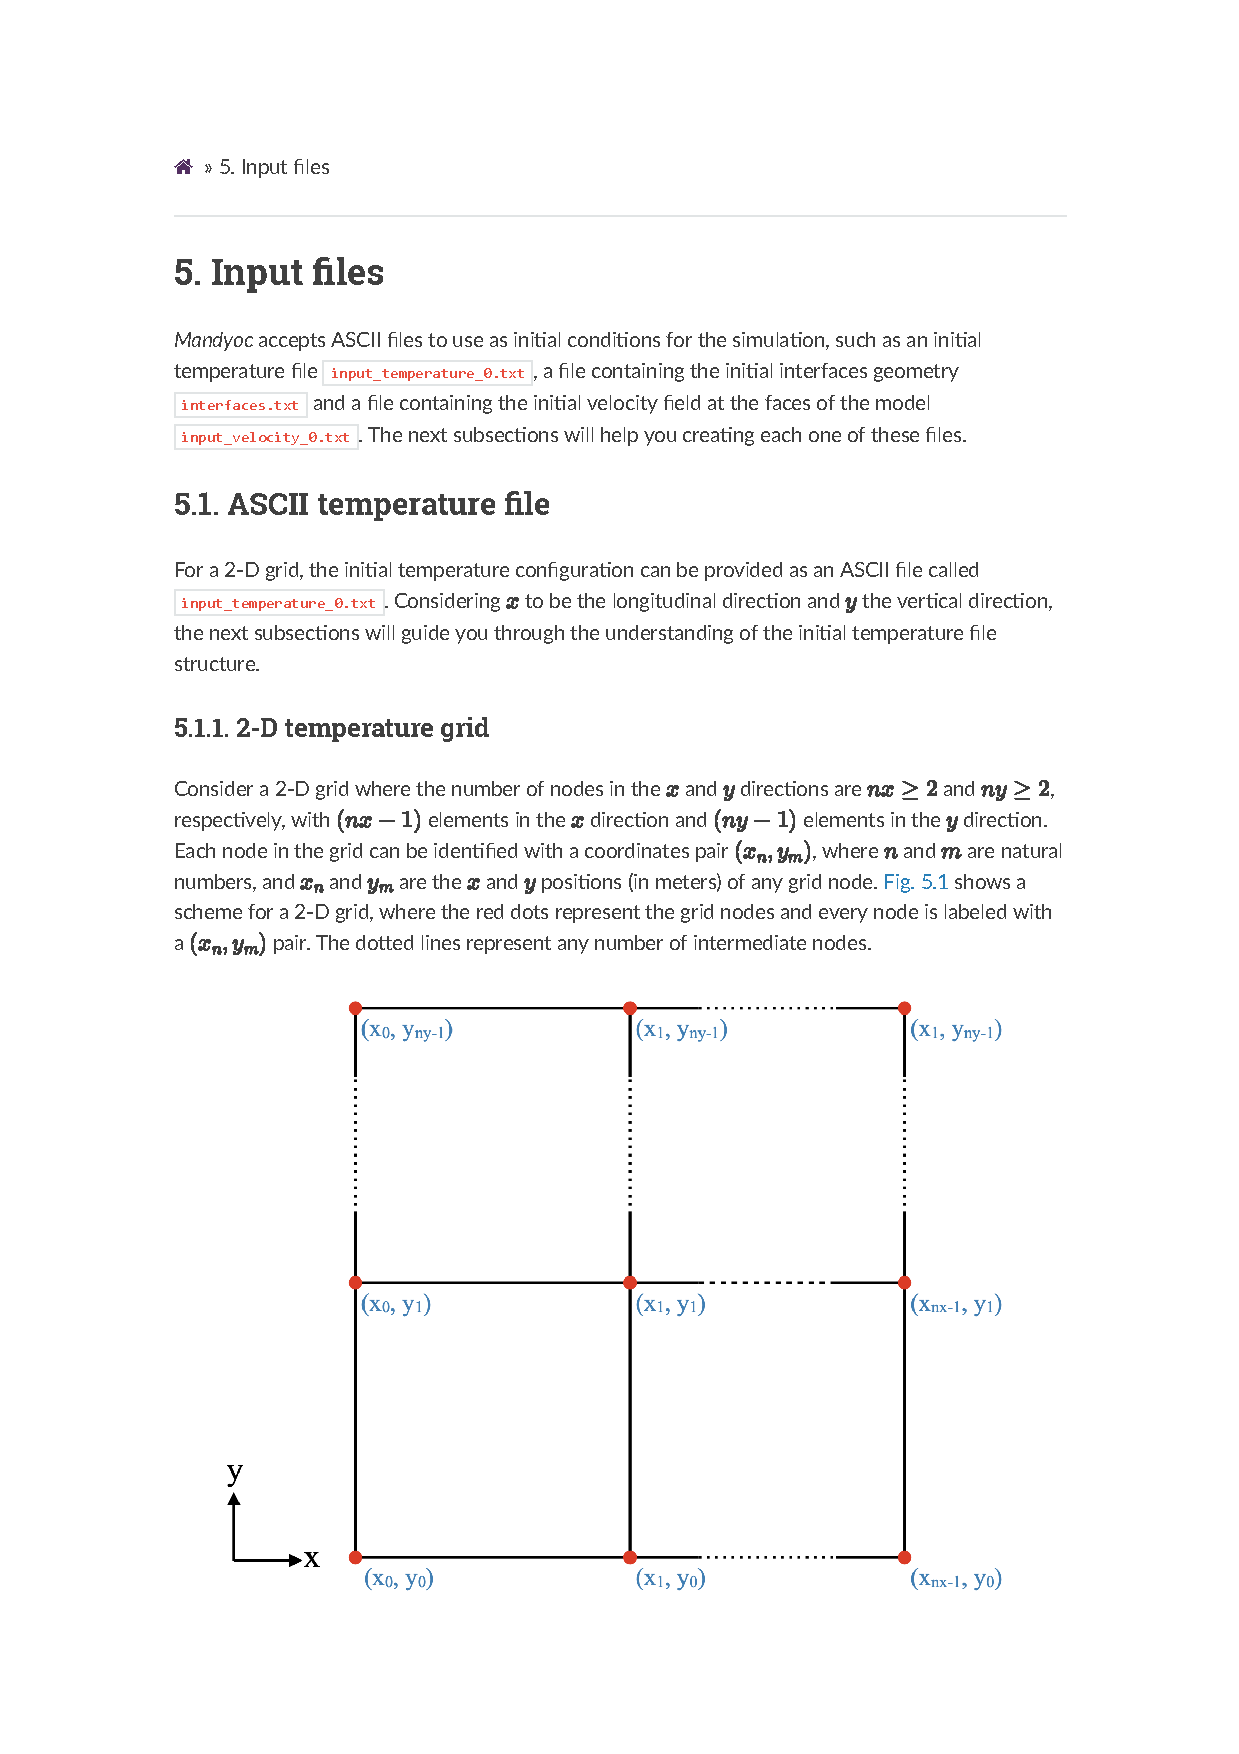
\includepdf[pages=-, scale=0.8, pagecommand={}, frame]{files/5.pdf}
% 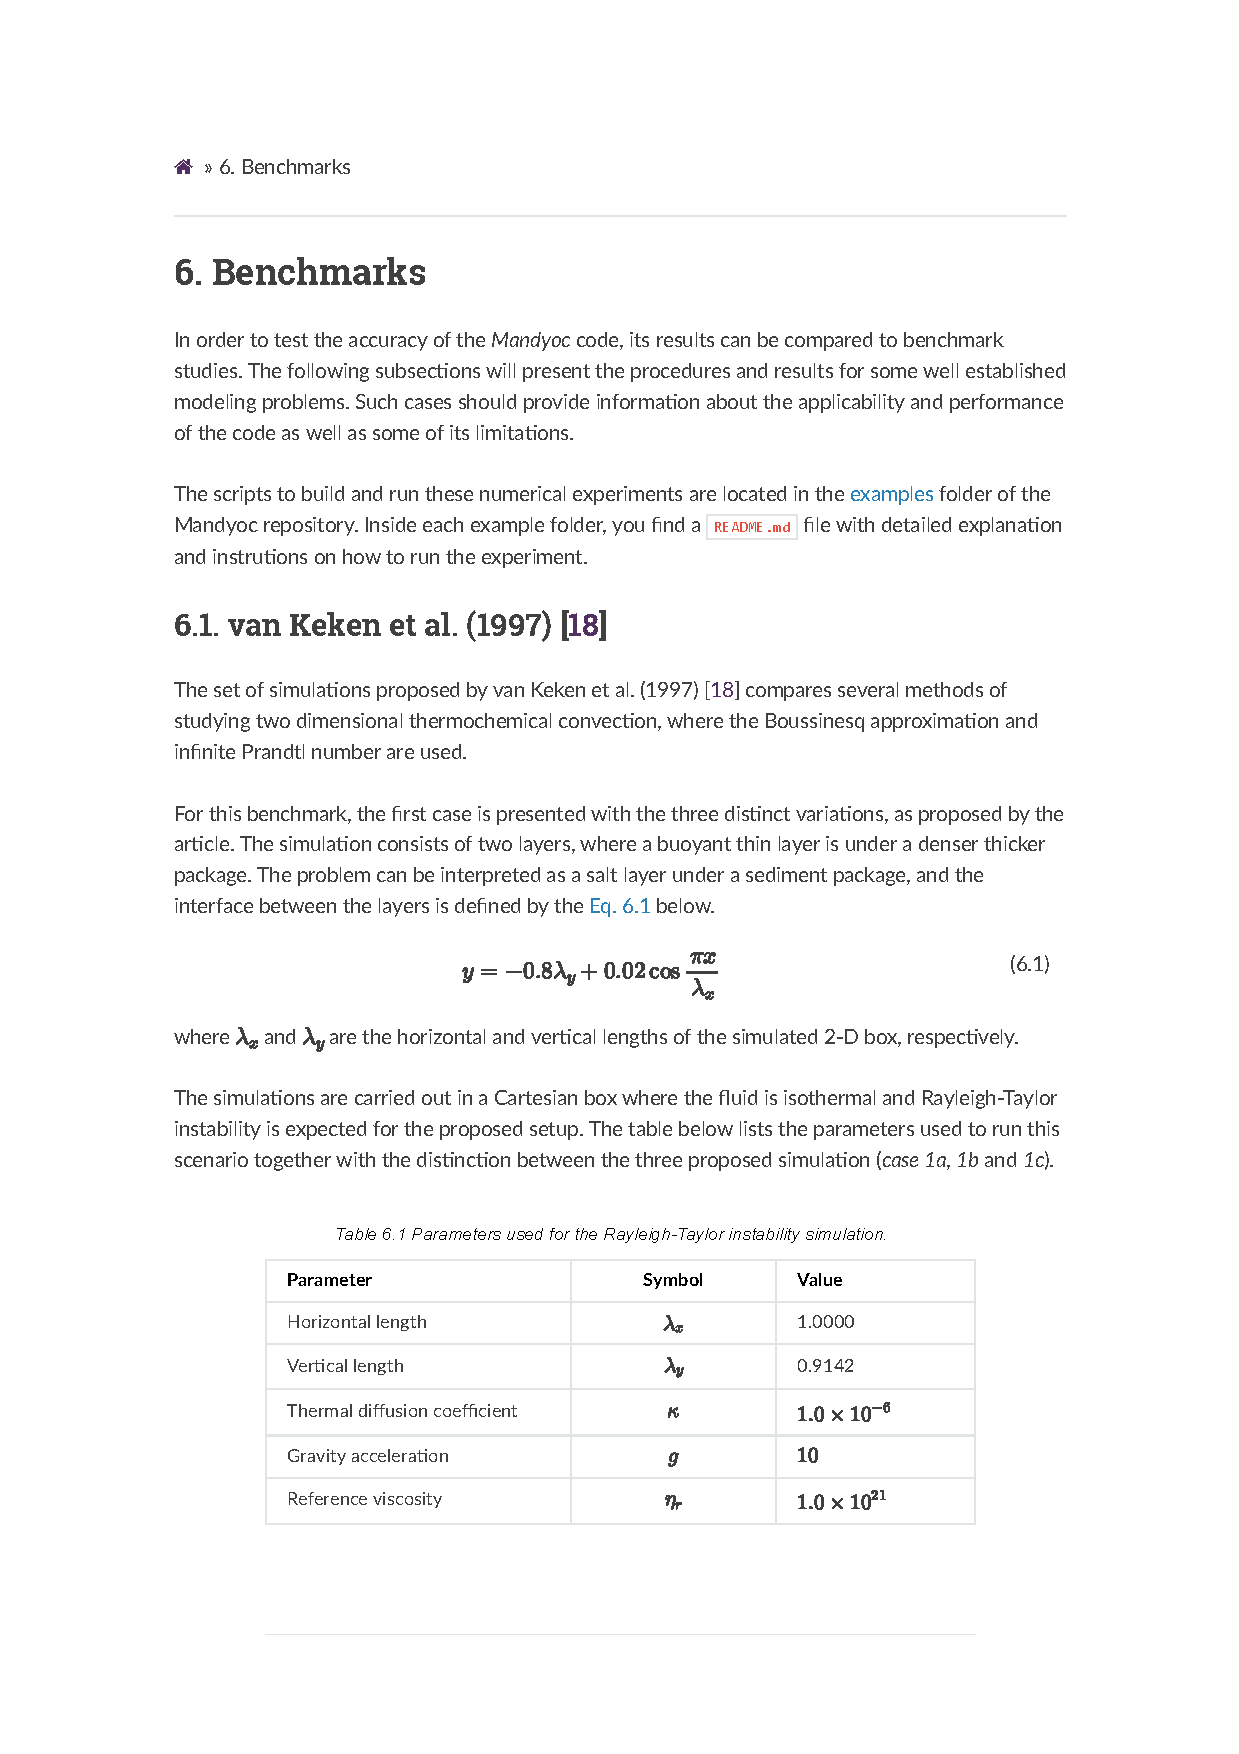
\includepdf[pages=-, scale=0.8, pagecommand={}, frame]{files/6.pdf}
% 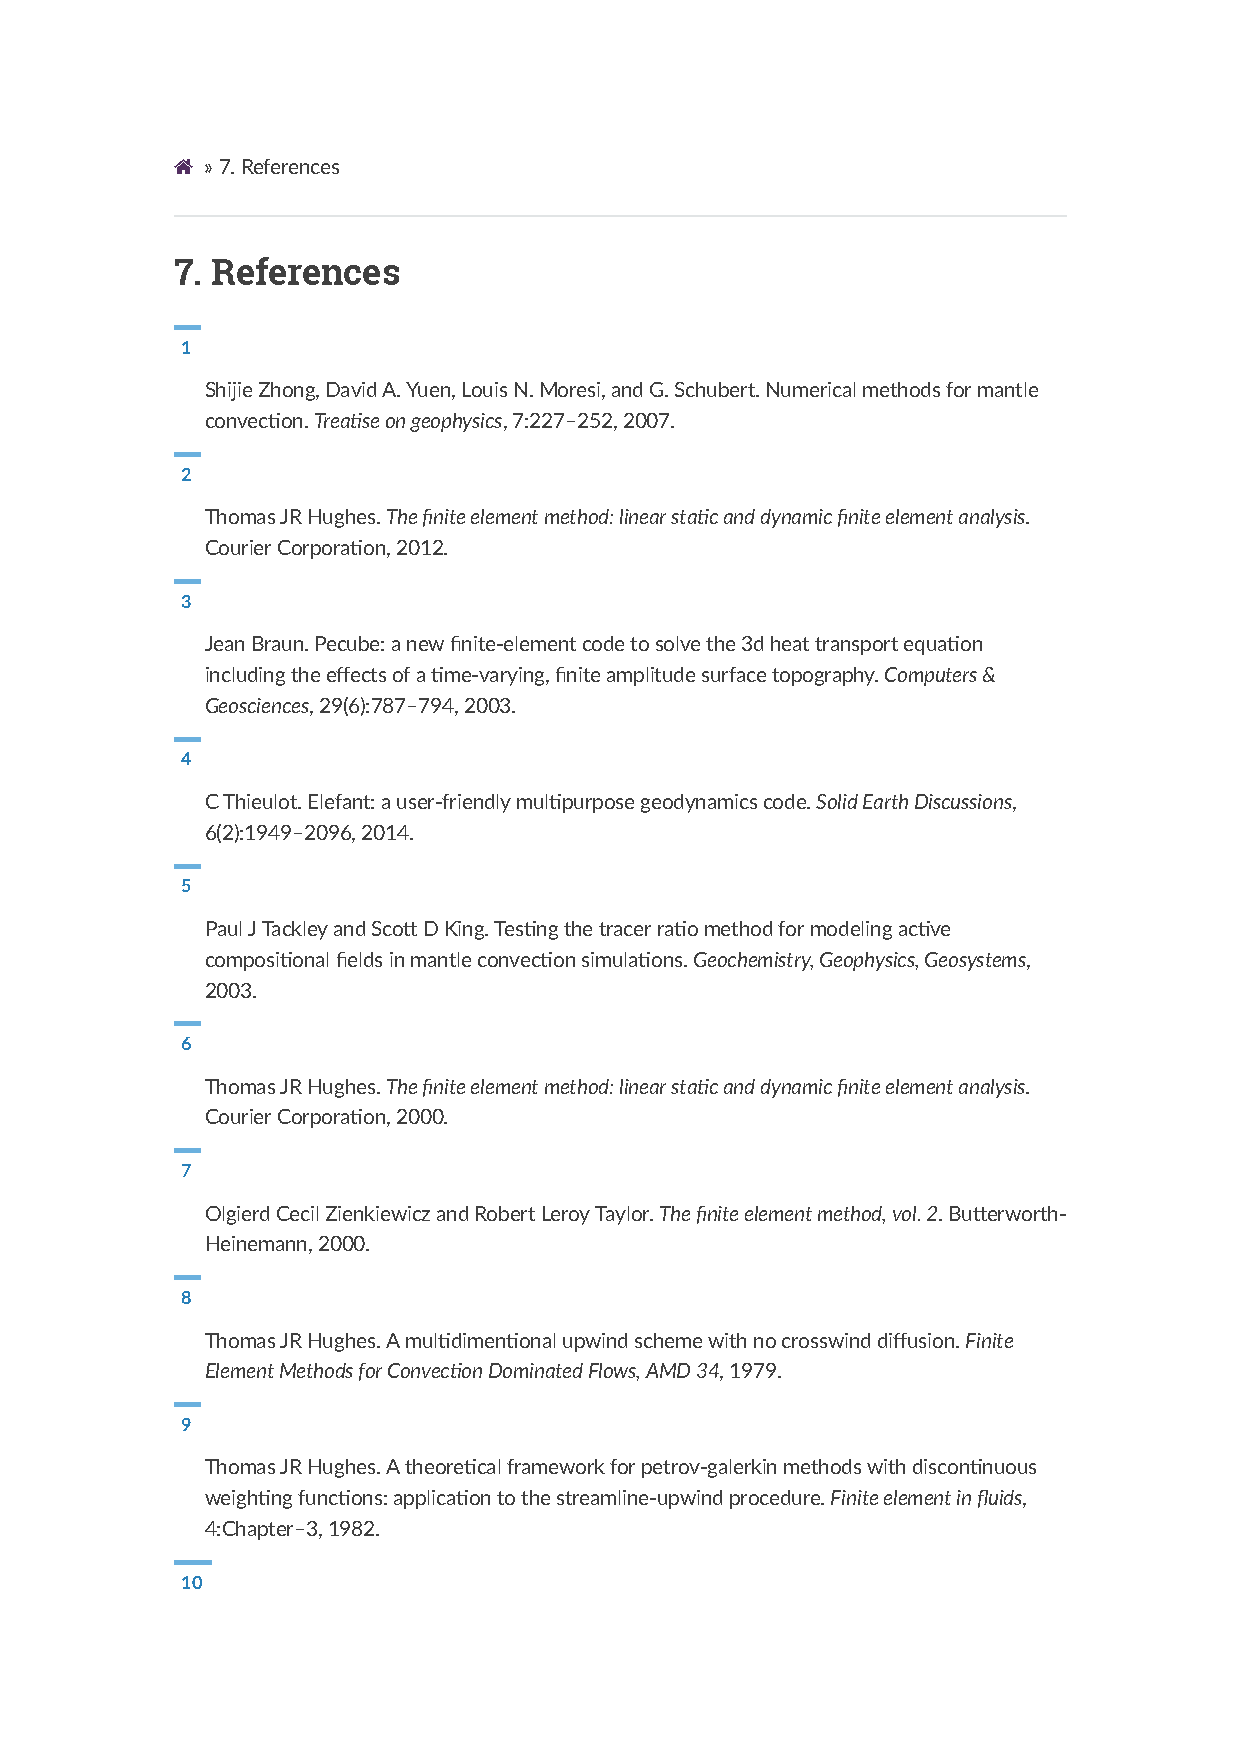
\includepdf[pages=-, scale=0.8, pagecommand={}, frame]{files/7.pdf}